\chapter{Android Aufnahmesystem}

In diesem Kapitel wird genauer auf das Android Aufnahmesystem eingegangen.

\section{Software Analyse}

\subsection{Anforderungen}

Um die Anforderungen zu evaluieren wurde das bestehende Aufnahmesystem auf Basis einer Nokia Symbian App analysiert. Alle vorhandenen Funktionen wurden erfasst und mit dem Industriepartner um weitere ergänzt. 
Eine kurze Übersicht über die bereits bestehenden Funktionen und den neu erfassten Anforderungen folgt in tabellarischer Form.

{\renewcommand{\arraystretch}{2}%
    \begin{longtable}{  p{3.5cm} | p{4.3cm} | p{4.3cm} }
    
    \textbf{Requirements} & \textbf{Altes System} & \textbf{Neues System} \\ \hline
\hline
    Positionsdaten übertragen & Geschwindigkeit, H\"{o}he, Richtung/Beschleunigung, Steigung, Longitude, Latitude & Geschwindigkeit, H\"{o}he, Richtung, Steigung, Longitude, Latitude \\ \hline
    Etappendaten & Zeit, Höhe, Distanz, Durchschnittliche Geschwindigkeit, UTC Zeit,Datum & Zeit, Höhe, Distanz, Durchschnittliche Geschwindigkeit \\
    \hline
     Tour Total & Zeit Total, Zeit Tour, Distanz Total, Distanz Tour, Höhe Total, H\"{o}he Tour & - \\
    \hline
    Netzdaten übertragen & Zellen ID, Location Area, Signal, Akku, Netzwerk, Netzwerk ID & Zellen ID, Area, Signal, Netzwerk ID, Technologie, Datenrate, RTT, Packet Loss\\
    \hline
    Bilder \"{u}bertragen & Bilder wurden \"{u}bertragen & Bilder werden \"{u}bertragen\\
    \hline
    Videostream \"{u}bertragen & Einzelne Bilder wurden \"{u}bertragen und serverseitig zu einem Stream zusammengef\"{u}gt & Videosequenzen werden \"{u}bertragen und serverseitig zu einem Stream zusammengesetzt\\
    \hline
    Anpassung der Bild- / Videoaufl"osung & - & Adaptive Angleichung der Auflo"osung an die verfu"ugbare Bandbreite\\
    \hline
    Lokales Caching & nur Bilder wurden gecacht & S\"{a}mtliche aufgenommene Daten werden lokal gespeichert\\
    \hline
	Aufnahme- systemstatus \"{u}bertragen & nur der Akkustand wurde an das Device Management Portal \"{u}bertragen & Detaillierte Statusinformation an das Device Management Portal\\
    \hline    
    Betriebsmodi & - & Managed - Einstellungen \"{u}ber das Portal / Unmanaged - Einstellungen am Ger\"{a}t\\
    \hline
	Auto-Start der App & - & App wird beim Ger\"{a}testart automatisch gestartet\\
    \hline    
    Externe Ger\"{a}te & ODB (Onboard Diagnose Bus) und Pulsinfo Ger\"{a}te wurden angesteuert & -\\
    \hline  
    Smartphone tauglich & Symbian App & Android App\\
    \hline 
    Log & Position und Bilder gesendet & Daten, Bilder, Status und Einstellungen gesendet / Exceptions\\
    \hline 
    Aufnahmestart Modi & Aufnahme hat automatisch bei App Start gestartet & Manuell, Zeitbasiert, Fernverwaltet oder bei Aktivierung einer externen Stromquelle\\
    \hline 
   	Power Management & - & Bei niedrigem Akkustand wird ein Energiesparmodus aktiviert\\
    \hline 
    Alarming Funktion & - & Treten Probleme aus, so wird darauf hingewiesen (z.B. keine GPS Daten w\"{a}hrend 2 Minuten)\\
    \hline 
    Mehrsprachig- keit & - & Deutsch und Englisch, einfach erweiterbar\\
    \hline 
    Fehlerkorrektur der GPS Daten & - & Ausreisser bei den GPS Daten werden herausgefiltert\\
    
    
\caption{Anforderungen Android Aufnahme System}
\end{longtable}}

Eine detaillierte Beschreibung aller Anforderungen befindet sich im Anhang. Folgend werden die aus unserer Sicht wichtigsten Anforderungen beschrieben.
%TODO referenz auf Anhang

\subsubsection{Funktionale Anforderungen}
\paragraph{Positionsaufnahme}
Die primäre Funktion des Aufnahmesystems besteht in der Aufnahme von Geopositionsdaten, deren Weiterverarbeitung und der Übermittlung an den TourLive Server. Über das GPS-Modul des Mobilfunkgerätes werden folgende Daten ermittelt:
\begin{itemize}
\item Aktuelle Position [GPS Longitude / Latitude]
\item Aktuelle H\"{o}he (GPS H\"{o}he) [m]
\item Aktuelle Zeit (GPS Timestamp) [unix\_time]
\item Geschwindigkeit (wird gelesen) [km/h]
\item Richtung (in Azimut, wird berechnet) [°]
\item Steigung (\"{u}ber die letzten 100m, wird berechnet) [%]
\item Anzahl Satelliten mit denen das Aufnahmeger\"{a}t verbunden ist
\end{itemize}

\paragraph{Bildaufnahme}
Ein wesentlicher Bestandteil des Aufnahmesystems ist die \"{U}bertragung von Bildmaterial in Form von einzelnen Bildern oder einem Videostream bestehend aus Videosequenzen. Folgende Funktionalit\"{a}t muss dabei beachtet werden:
\begin{itemize}
\item Anpassung der Bildaufl\"{o}sung adaptiv an die verf\"{u}gbare Datenraten (optional)
\item Bilder sollen automatisch, in der korrekten Ausrichtung an den Server geschickt werden (Stichwort Ger\"{a}tesensoren)
\end{itemize}


\subsubsection{Nichtfunktionale Anforderungen}

\paragraph{Sicherheit}
In Bezug auf Vertraulichkeit und Integrit\"{a}t werden keine speziellen Anforderungen gestellt. Die Daten\"{u}bertragung erfolgt unverschl\"{u}sselt. Das Aufnahmeger\"{a}t muss sich am TourLive Server nicht explizit authentisieren. In Bezug auf Verf\"{u}gbarkeit sind die Anforderungen hoch. W\"{a}hrend dem Rennen soll es keine L\"{u}cken ohne Daten von mehr als 5 Minuten geben. K\"{o}nnen w\"{a}hrend einer bestimmten Zeitspanne keine Daten \"{u}bertragen werden, sollen diese gepuffert und zu einem sp\"{a}teren Zeitpunkt \"{u}bertragen werden. 

\paragraph{Ausfallsicherheit}
Die gesammelten Daten (Positionen, Bilder,..) werden parallel auf dem lokalen Ger\"{a}tespeicher abgelegt. Erreicht dieser 80\% der verf\"{u}gbaren Kapazit\"{a}t werden automatisch alte Eventdaten gel\"{o}scht. Über dieses lokale Caching wird sichergestellt, dass die  gesammelten Daten aufgrund technischer Probleme bei der Daten\"{u}bertragung nicht verloren gehen. 

\subsection{Technologien}

\subsubsection{Android}
Die native Programmiersprache f\"{u}r das Android Betriebssystem ist Java. Die Programmierung in Java bringt den Vorteil, dass auf die gesamte Application Programming Interface (API) von Android zugegriffen werden kann. Weiter sind die Ger\"{a}te genau dafu\"{u}r ausgelegt und eine optimale Performance kann erreicht werden. S\"{a}mtliche Komponenten dieser Arbeit sind in Java geschrieben.

\subsubsection{Externe Libraries}
Um den geforderten Funktionsumfang umzusetzen nutzt die Applikation folgende zwei externe Libraries.
\paragraph{Spring for Android\footnote{Spring for Android, \url{http://www.springsource.org/spring-android}, aufgerufen am 29.04.2013} }
Ein Rest Client für Android von den Entwicklern des populären Java Spring Frameworks. Der Rest Client bietet einfache Deserialisierung eines JSON-Strings in ein Java Objekt. Diese Library wird benötigt um die Kommunikation zwischen dem Aufnahmesystem und den beiden Serversystemen zu ermöglichen.
\paragraph{ORMLite\footnote{ORMLite, \url{ormlite.com}, aufgerufen am 02.05.2013}} ORMLite ist eine OpenSource Java Library, welche das Objectrelational mapping
(ORM) übernimmt. ORMLite bietet eine speziell auf Android angepasste Distribution.\\
Um eine Klasse mit ihren Feldern zur Persistierung zu markieren, werden Java Annotationen verwendet. Aus diesen Annotationen erstellt ORMLite die Datenbank. Darüber hinaus werden mit ORMLite alle Zugriffe auf die SQLite Datenbank ausgeführt. In dieser Arbeit wird die ORMLite Version 4.45 verwendet. Diese Library wird verwendet um die gesammelten Informationen lokal in einer Datenbank speichern zu können und um somit die Datenkonsistenz bei Verbindungsunterbrüchen sicherstellen zu können.

\subsection{Entwicklungsumgebung}
Die von Android empfohlene Entwicklungsumgebung ist Eclipse\footnote{Eclipse, \url{http://eclipse.org}, aufgerufen am 29.04.2013}  mit einem Plugin zur Entwicklung von Android Applikationen. Auf der Entwicklerseite von Android steht dazu folgendes:
\begin{quotation}
Android Development Tools (ADT) is a plugin for the Eclipse IDE that is designed to give you a powerful, integrated environment in which to build Android applications.\footnote{Android Plugin f\"{u}r Eclipse, \url{http://developer.android.com/tools/sdk/eclipse-adt.html}, aufgerufen am 29.04.2013} 
\end{quotation}
Eclipse ist eine weit verbreitete IDE und wird aktiv weiter entwickelt. Mit dem Plugin zusammen bildet sie eine solide Grundlage f"{u}r dieses Projekt.
Damit die Android Applikation direkt auf dem Computer getestet werden kann, stellt Google einen Emulator zur Verf"{u}gung. Der Emulator ist allerdings auch als solcher zu betrachten, da die Bedienung nicht vergleichbar mit einem richtigen Smartphone ist.

\paragraph{Android Version}
Eine Anwendung wird f"{u}r eine spezifische Android Version entwickelt und getestet. Somit kann garantiert werden, dass das Verhalten der Anwendung immer gleich ist. In dieser Arbeit ist dies die Version 4.0 mit dem Versionsnamen Ice Cream Sandwich\footnote{Android Ice Cream Sandwich, \url{http://www.android.com/about/ice-cream-sandwich/}, aufgerufen am 29.04.2013}.
Die Entwicklung auf einer Version schliesst jedoch nicht aus, dass die Anwendung in neueren Versionen nicht mehr lauff"{a}hig ist.

\subsection{Paper Protoypes}
Nach dem die Anforderungen definiert waren, haben wir Paper Prototypes erstellt. Diese wurden mit dem Industriepartner besprochen. So konnten mögliche Missverständnise eliminiert werden. Hier eine Übersicht über alle erstellten Mockups. Eine genauere Beschreibung befindet sich im Anhang.

\begin{figure}[H]
	\centering
	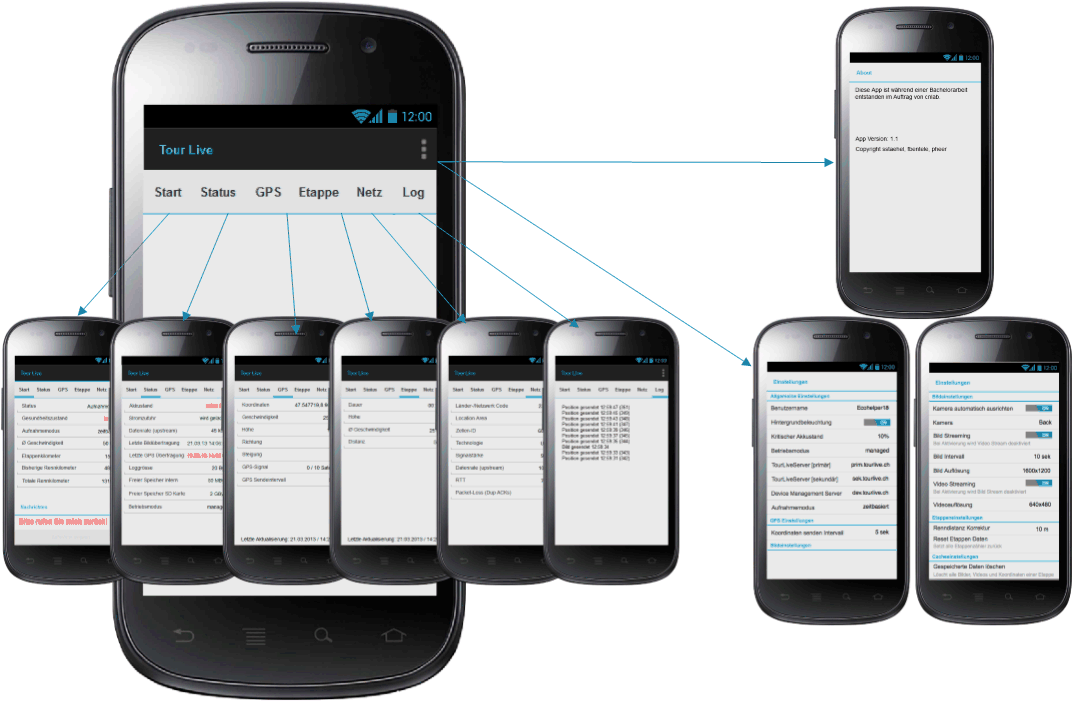
\includegraphics[width=150mm]{images/android/OverviewAndroid.png}
	\caption{Übersicht Android Mockups}
\end{figure}

\subsection{Domain Model}


\section{Software Design}
\subsection{Architektur und Übersicht}
Die Android Applikation sammelt Daten für die beiden Server. In der Abbildung ??? %TODO 
 wird veranschaulicht, welche Daten an welchen Server verschickt werden.

\begin{figure}[H]
	\centering
	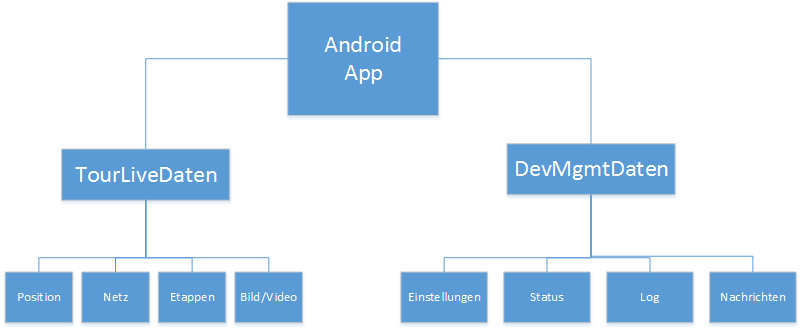
\includegraphics[width=120mm]{images/android/uebersicht.png}
	\caption{Grobstruktur der Android App}
\end{figure}


\subsubsection{Architekturentscheide}

\paragraph{Caching}
Um sämtliche aufgenommene Daten zu Cachen, haben wir uns für die Objektrelationale Abbildung der Klassen in der SQLite Datenbank entschieden. Dies ermöglicht mit Annotation eine schnelle Einbindung. Alternativen wären die Speicherung in ein Textfile oder die Speicherung in der Datenbank ohne Objektrelationale Abbildung, jedoch stand beides nicht zur Diskussion, da sie einem ORM gegenüber viele Nachteile bringen.

\paragraph{Datenhaltung}
Um die verschiedenen Services und Container überall zur Verfügung zu haben und somit lange Aufrufketten zu verhindern, wurde ein Singleton Repository eingeführt. In diesem Repository können über Methoden auf alle Daten zugegriffen werden, die von diversen Klassen gebraucht werden.

\paragraph{TourLiveApplication}
Beim Start der Applikation müssen viele Daten initialisiert werden. Um dies bereits zu machen, bevor eine View geladen wurde, wurde eine TourLiveApplication erstellt, welche von der Android Klasse Application abgeleitet wird. 

\paragraph{Berechnungen}

\subsection{Schichtenmodell und Paketdiagramm}
Die Android Applikation teilt sich in 3 Schichten auf.

\begin{figure}[H]
	\centering
	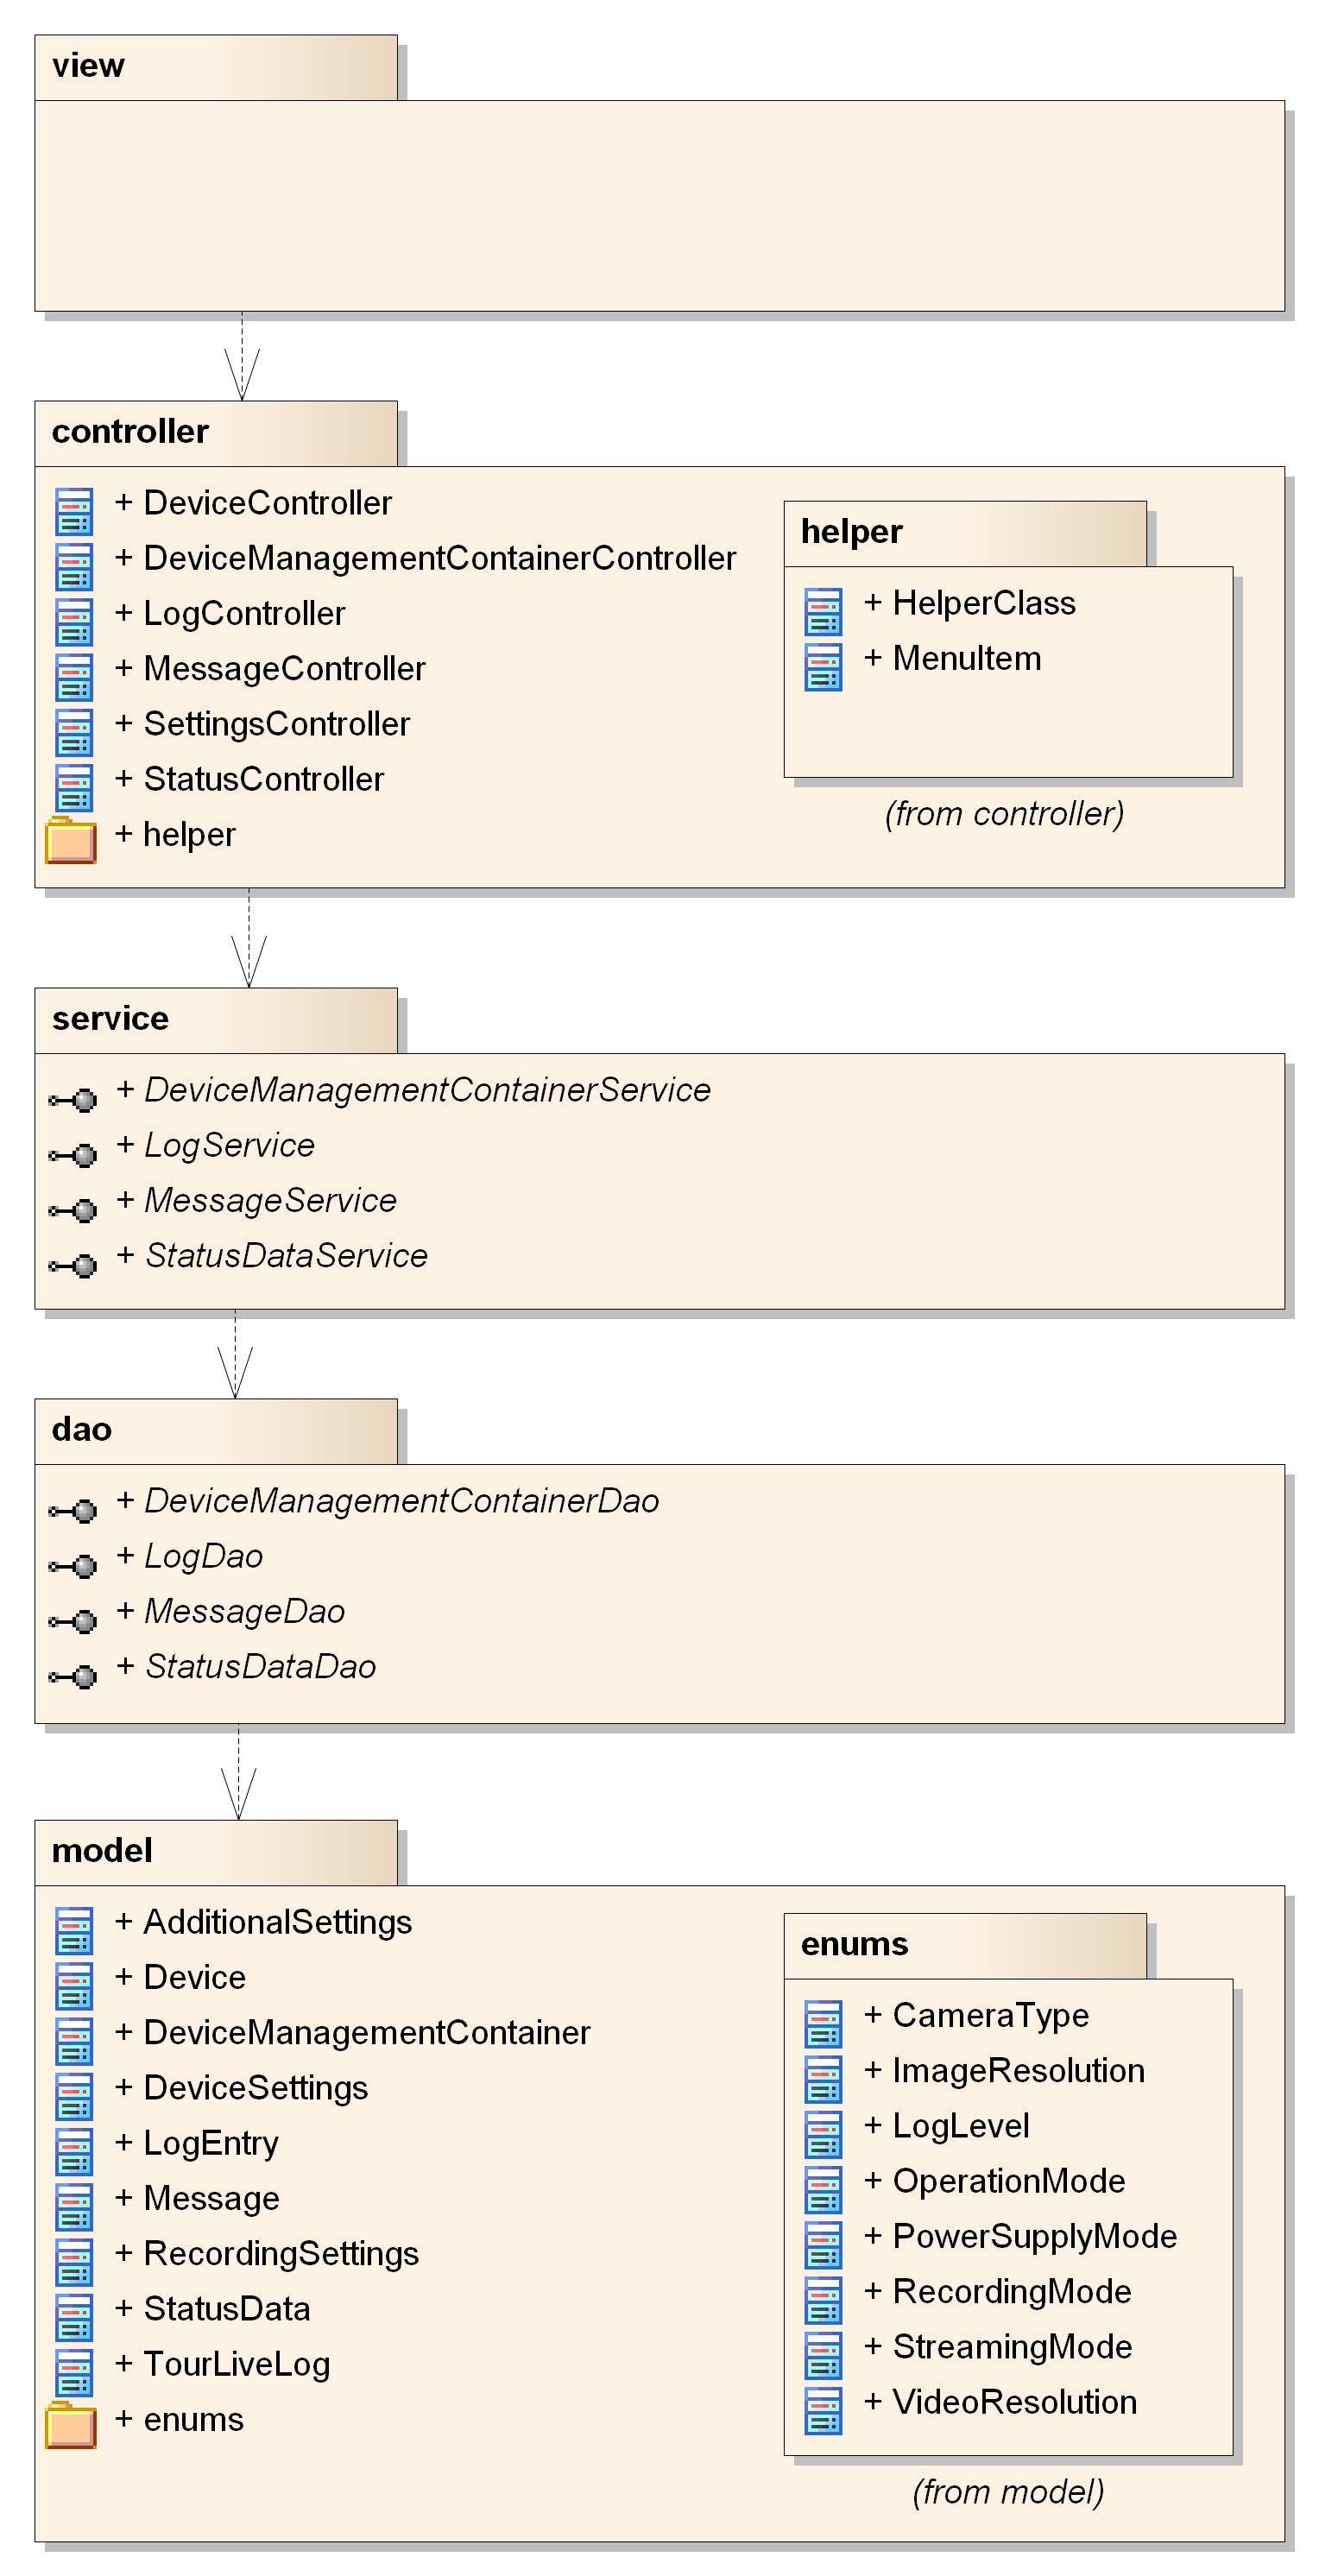
\includegraphics[width=150mm]{images/tourliveweb/schichten.jpg}
	\caption{Packagediagramm des Aufnahmesystems}
\end{figure}

Die oberste Schicht stellt die Schnittstelle zum Benutzer dar. Diese Klassen sind für die Darstellung zuständig.\\
In der nächsten Schicht ist die ganz Businesslogik enthalten. Hier werden bei einer Aufnahme alle Timer gestartet und verwaltet und die jeweiligen Aktionen ausgeführt. \\
In der letzten Schicht enthält die Domäne des Aufnahmesystems.

\section{Realisierung}